%% Los cap'itulos inician con \chapter{T'itulo}, estos aparecen numerados y
%% se incluyen en el 'indice general.
%%
%% Recuerda que aqu'i ya puedes escribir acentos como: 'a, 'e, 'i, etc.
%% La letra n con tilde es: 'n.

\chapter{Requirements}
\newpage

This chapter exposes the requirements acquired after analysing the needs of the users. This analysis is required before the design of the system.\\

This analysis implies to organize several meetings to obtain the needs of the the users that were going to use the system. Listen to the needs of the client is required to look for a good solution to the main problem.\\

The solution was obtained after doing a good analysis of the tools available to develop the Information System. This solution is not unique, there are more available solutions, but in this project, we decided to developed the purposed solution because it was affordable in terms of time and budget.

\section{User requirements}

This section explains the process followed to obtain information about the needs of the user. Here it is explained how the process was made and the steps that we followed to get the information to develop the purpose system.\\

To do this process, it was needed to organize meetings with one of the potential users of the system. Several meetings were needed to obtain all the requirements of the system. There are an amount of questions to obtain the requirements of the users. These questions are described in the following points:

\begin{itemize}

\item \textit{What does the user need?} The most relevant question asked to the user. We need to know exactly the desires of the user to check the requirements and, after that, decide if the project is affordable or not.

\item \textit{Who is going to use the system?} This question is required to obtain the profiles of the users that are going to use the system. The experience of the user is considered to develop an appropriate solution. With this information we have an idea about the knowledge of the users and how must be the system for the different users that are going to use it.

\item \textit{When does the user want to get the results?} This question is used when there is a limited requirement related to time. Above all, there is a limit of time established by the user.

\item \textit{How does the user want the results?} The user explains how must be the results. Also, the format to display the information is considered.

\item \textit{Where does the user want to have access to the system?} Here, it is defined if the system has to be accessible from everywhere or not.

\item \textit{Why does the user need the system?} This is the main reason to analyze if the purposed solution fits to the needs of the client.

\end{itemize}

The engineer has to asks all these questions to acquire the requirements of the client. The answers to these questions are exposed in the following points:

\item \textit{What does the user need?} The user needs a system to monitore the measures of soils. The system has to be easy to use and automated.

\item \textit{Who is going to use the system?} The system is destinated to users who are going to study soils. These users have a medium knowledge managing \textit{Information Systems}.

\item \textit{When does the user want to get the results?} The results have to be displayed in Real Time.

\item \textit{How does the user want the results?} There is no prefered way to display the results. The format of the results have to be compatible with \textit{Microsoft Excel}.

\item \textit{Where does the user want to have access to the system?} There is no limitimation for this requirement, but mobility is a relevant feature to add to the system. Wireless solutions are considered to implement this feature.

\item \textit{Why does the user need the system?} Conventional solutions produces results depending on long time processes. This system allows to have an overview of the measures in \textit{Real Time}. The calculates are produced faster with this system.

After obtaining the answers to all these questions, we have an idea about how must be the system the users want. In this study, the user wants a customized and simple system to query information about materials and to get fast results to do analysis.\\

It is considered an affordable project because the available technology provides a potential solution to solve the main problem discussed in this document.

\subsection{Measure requirements}

The specifications of the measures have to be defined. The user gave some information about the available sensors that could be used to develop the required system.\\

The user does not need complex sensors, the user wants to estimate information and compare the results with other technologies available in the market.\\

The information measured by the sensors must be accessible for all the users. This information has to be interpreted with known values to use it for other studies. The interpretation of the values must be considered, the measures are linked to real percentages of humidity.

\subsection{Access requirements}

The system has to be accessible for the users that are going to use the system. The access to the system and its limitations have to be explained.\\

Mobility and comfort are other requirements to consider. The system has to be accessible from different devices (e.g. computers, mobile phones or tables).\\

To satisfy this requirement it was established a wireless network to allow the access to the information obtained by the system. This requirement makes the system flexible.

\subsection{Functionality requirements}

The system has to monitor the information registered from sensors in Real Time. The system has to be available every time.\\

The information of the studied materials is registered. The objective of monitoring during long period of times is to obtain precise results in the studies. When the measures increase the predictions adjust better to real values.\\

The control of the system allows to detect possible issues on it (e.g. the system crashes). Also, the issues are tracked to fix them easily.

\section{Technical requirements}

This section is dedicated to describe the requirements related to the physical system and the technology used to develop the purposed system.\\

Here there is an explanation about why it was decided to use the technology described and the features of the designed system. This information makes easier to decide which technology is appropriated to design the system.\\

The designer has to think if the chosen technology satisfies the requirements of the users.

%% Continue here

\subsection{Hardware requirements}

This section is dedicated to explain the requirements of the hardware used by the system.\\

The hardware has to be simple to use and transparent for the users. The users do not mind the election of the designer, they just want to use the system and do their work as better as possible.\\

The hardware has to be configurable because the user has a customized configuration to work. It should respond to the needs of the users.\\

The selected hardware has to have an easy deployment. It should be deployed everywhere, although the conditions are not the best for a normal system. The system has to work normal although there are in the ambient dust, noise or different item that can make interferences in the system.

\subsection{System requirements}

The system has to be accessible for the users. The user can query information without having a knowledge about how the systems works internally. The user does not need to configure anything in the system.\\

The system has to be auto-configured when the user wants to use it. It implies that it should be automatized and prepare to work every-time and every-where.\\

An important feature of the system is easy way to upgrade and its management. The system should be prepared for improvements if the user needs to upgrade it.

\subsection{Software requirements}

The software has to work transparently to the user. The user must not know how it works internally.\\

The software obtains information about some sensors. It stores the information into a system that is able to manage information. This information is accessible to the user. Also, the information is interpreted according to the requirements of the user.\\

It should be improvable and upgradeable if the needs of the users change.

\section{Planning used in this project}

One of the most important things needed to consider in a project is the existence of a Project Management. In this project, it was required to plan different scheduled meetings (to know the needs of the client), calculate timings related to investigation and analysis of the different alternatives which are interesting to apply to this project. Also, considering different death lines it is a relevant requirement (e.g. implementation plan).\\

It was considered the time needed to maintain the system after finishing its deployment and how to prepare the client to use the deployed system. Although the client has his knowledge to use the system, it was inevitable to invest efforts to prepare a good documentation to allow to future developers to improve and to manage the full system.\\

If we have to enumerate the different things we needed to consider, the most important points are the following:

\begin{itemize}
\item Time needed to know the needs of the client.
\item Time inverted to invest the correct technology to develop the system.
\item Time inverted to get all the components needed to develop the system.
\item Time inverted to develop a correct implementation plan.
\item Plan different meetings to expose the status of the project.
\item Time needed to develop the solution chose by the stakeholder and the engineer.
\item Resources used to deploy the system.
\item Study the results obtained by the developed system.
\item Time inverted to form the client to use the system.
\item Time inverted to provide a good documentation to the client.
\item Time inverted in tasks related to the maintain of the working system.
\end{itemize}

\subsection{Software development methodology used in this project}

Before starting to plan all the tasks needed to develop the \textit{Measure System}, it was invested efforts to decide which methodology fits better to this project. There are several methodologies we can apply to start the development of this project. The different methodologies we could apply to this project are the following:

\begin{enumerate}

\item Waterfall development. It was discarded since the beginning because the client provides low feedback. This methodology was not the correct one for this project because. The client has to know what is done in the project and the client has to participate in the development plan.

\begin{figure}[H]
\begin{centering}
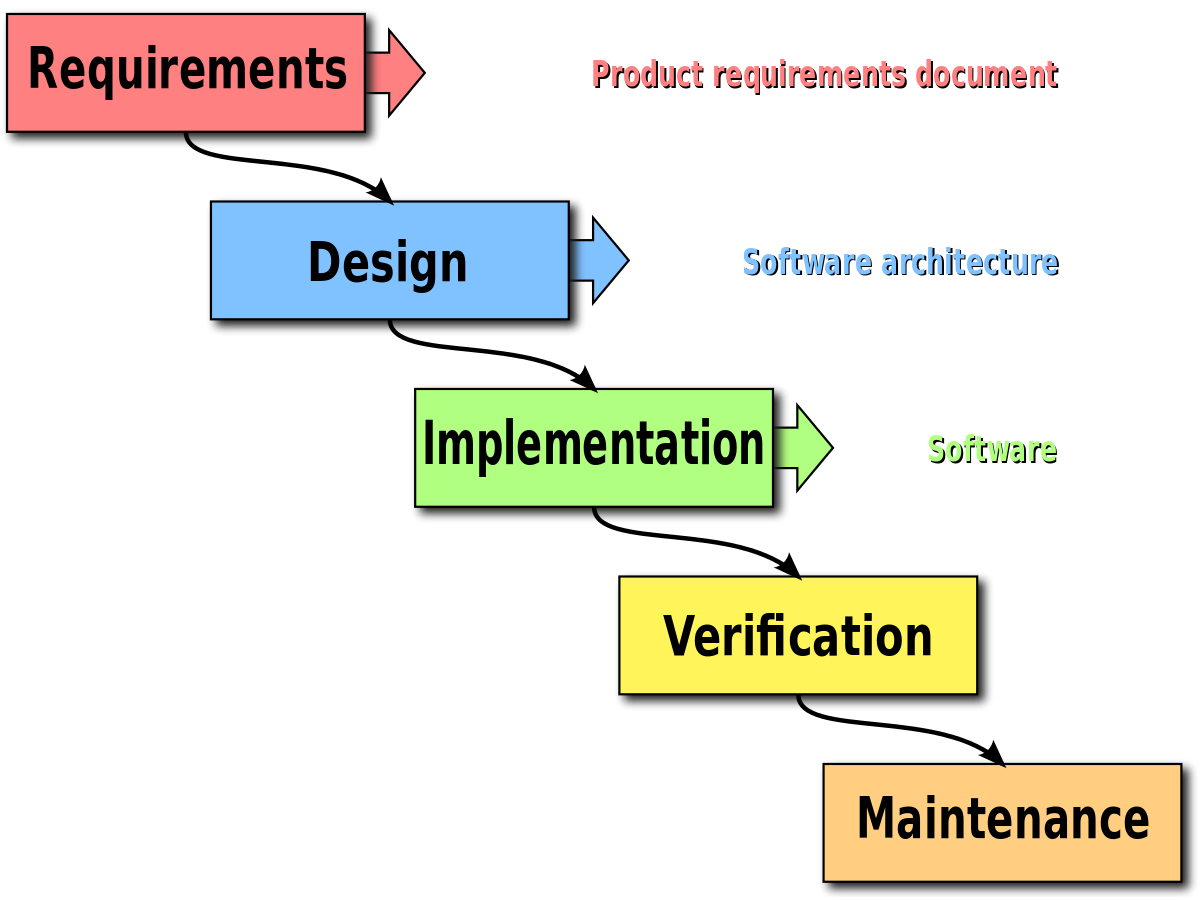
\includegraphics[scale=0.2]{IMGS/waterfall_methodology.png}
\caption{Waterfall methodology \label{Waterfall methodology}}
\end{centering}
\end{figure} 

\item Spiral development. It is an interesting methodology because all the phases of the project are reviewed in all the steps, improving the quality of the final product. The weakest point of this methodology is that the client sometimes cannot participate in the development plan.

\begin{figure}[H]
\begin{centering}
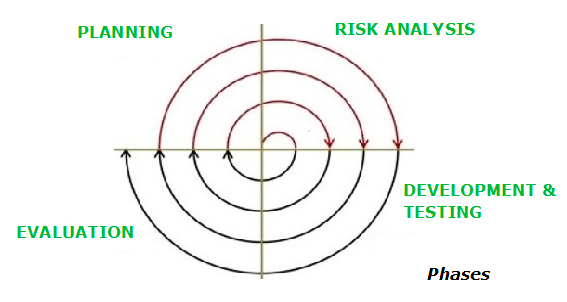
\includegraphics[scale=0.5]{IMGS/spiral-model.jpg}
\caption{Spiral model \label{Spiral model}}
\end{centering}
\end{figure} 

\item V-Model. It is similar to the Spiral development but it has the inconvenient of the cost associated when it is required to change features which took place at the beginning of the project. Things are changed when the project or the step is in the final state and it has a high cost when it is needed to apply modifications.

\begin{figure}[H]
\begin{centering}
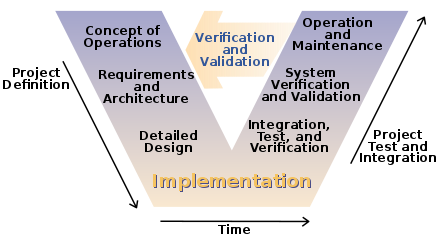
\includegraphics[scale=0.5]{IMGS/v_model.png}
\caption{V model \label{V model}}
\end{centering}
\end{figure} 

\item Scrum. This is one of the fittest methodologies we can apply to this project. The best characteristic of this methodology is that the client can participate in the development process of the product. It is flexible and the costs associated to changes are not high.

\begin{figure}[H]
\begin{centering}
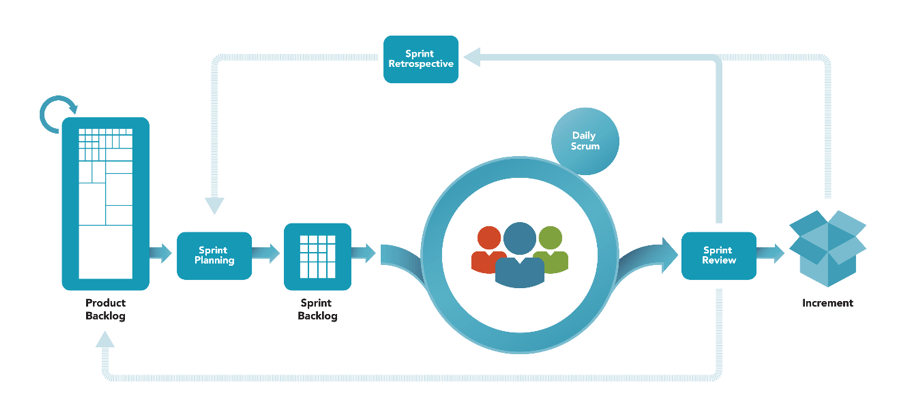
\includegraphics[scale=0.5]{IMGS/Scrum.png}
\caption{Scrum methodology \label{Scrum methodology}}
\end{centering}
\end{figure} 

\end{enumerate}

After knowing the different methodologies we could apply to this project, it was decided to use a hybrid between Spiral development and Scrum model. The main reason to combine both methodologies is the possibility to review the project in every step and the importance of the participation of the client in the project. The most important thing is to consider the opinion of the client in every steps because the client is the person which can allow us to develop the correct solution to his/her needs.\\

The other methodologies are not the correct ones to apply to this project because it is more difficult to allow the client to participate in the different phases of the project.

\section{Project Management}

This section of the memory exposes the distribution of the tasks in terms of time and budget. The resources used to develop the system are considered too to calculate the total budget of the project. The budget represents the value of the resources in euros per hour. Also, there are resources which have a fix value which does not depend on time (physical components). The planning used to carry out this project is based on the time required to approach the tasks which were defined at the beginning of the project.\\

\subsection{Resources}

Resources are the assets required to approach a project. The cost of the resources is disparate, depending their value over time. The most relevant resources of this study are described in the following points:

\begin{itemize}

\item Value of the workforce. The workforce is calculated based on the price per hour of the employee. The student is considered as an employee which earns money based on his effort. The effort is associated to the time invested to work on a determined task. The cost of the effort is measured by euros per hour.
\item Hardware components. These components have a fix price set by the provider of the products.

\end{itemize}

The resources of this project are represented in the following picture.

\begin{figure}[H]
\begin{centering}
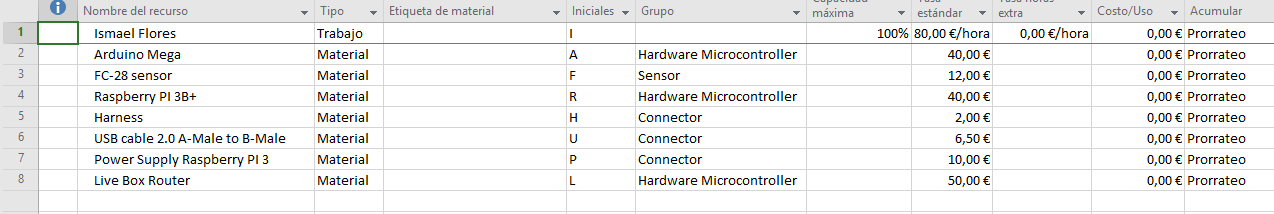
\includegraphics[scale=0.5]{IMGS/resources_project.PNG}
\caption{Resources of the project \label{Resources of the project}}
\end{centering}
\end{figure}

The picture includes the information of the selected employee to approach the project and the different materials required to develop the purposed Information System.

\subsection{Distribution of the tasks}

To approach this study, it was required to distribute the detected tasks of the project. There are several task to perform and they represent the different phases of the project.\\

It was estimated that the time required to develop the system is approximately \textit{352 hours} following the calculates of the project management phase. This section explains the biggest phases of the project although they are divided in subphases. The most important tasks are described as follows:

\begin{itemize}

\item \textit{Requirements}. This task represents the invested time to acquire the requirements of the client. During this task, it was defined the structure of the project, the requirements of the user and the requirements of the system. This task represents the 30\% of the project. The total of hours invested to this phase is \textit{96 hours}.
\item \textit{Design}. This task includes the process invested to design the purposed system based on the requirements of the user. Here, the architecture of the system is defined according to the different components of the system. This task represents the 20\% of the effort of the project. The amount of hours of this phase is \textit{64 hours}.
\item \textit{Development}. Includes the tasks related to the implementation of the system according to the requirements and the design of the system. This tasks invests the 30\% of the effort of the project. The amount of hours dedicated to this phase is \textit{96 hours}.
\item \textit{Testing}. The tasks related to testing checks if the developed system complies with the requirements of the client. Performance and stability are considered too. Also, the deployment of the system is approached in this phase of the project. It represents the 10\% of the effort of the project. This phases takes the smallest time invested, considering for this phase \textit{32 hours}.
\item \textit{Maintenance}. This phase of the project takes of the system detecting possible issues and improving the features of the system. This phase represents the 20\% of the effort of the project. The dedication to this phase represents a total of \textit{64 hours}.

\end{itemize}

The information commented before explains how is the distribution of the tasks and the percentage of time invested in all of them. In the following picture, it is provided the information of the phases of the project. All the phases depend on time. The information of all the tasks is displayed in the following Gantt's diagram.\\

\begin{figure}[H]
\begin{centering}
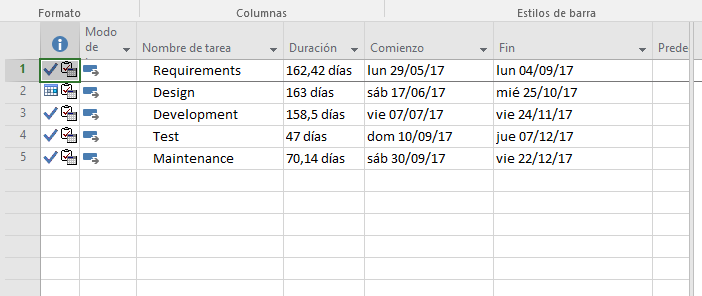
\includegraphics[scale=0.8]{IMGS/gant_chart.PNG}
\caption{Gantt's diagram of the project 1/2\label{Gantt's diagram}}
\end{centering}
\end{figure}

\begin{figure}[H]
\begin{centering}
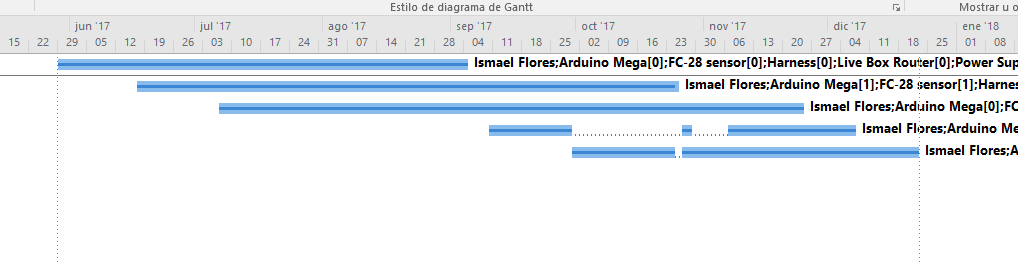
\includegraphics[scale=0.6]{IMGS/gant_chart2.PNG}
\caption{Gantt's diagram of the project 2/2\label{Gantt's diagram}}
\end{centering}
\end{figure}

The information displayed in the Gantt's diagram shows the time invested in all the tasks of the project. The time invested for all the tasks is represented by days. The project starts at \textit{29\begin{small}th\end{small} of May of 2017} and finishes at \textit{22\begin{small}nd\end{small} of December of 2017}. The time invested in all the tasks considered in days is the following:

\begin{itemize}

\item \textit{Requirements}. An amount of 162 days are required to finish all the subtasks related to requirements.
\item \textit{Design}. An amount of 162 days are required to finish all the subtasks related to design.
\item \textit{Development}. An amount of 158 days are required to finish all the subtasks related to development.
\item \textit{Testing}. An amount of 47 days are required to finish all the subtasks related to testing.
\item \textit{Maintenance}. An amount of 70 days are required to finish all the subtasks related to maintenance.

\end{itemize}

The graph displays how the testing phase was sectioned. The testing phase was carried out every-time there was a new release of the software. The testing phase detects if there are bugs in the system, and in case there are bugs, they are reported to fix them in the next release.

\subsection{Cost of the project}

This section exposes the cost associated to the project. Here, there is an explanation about the cost of the available resources of the project.\\

After preparing the project management, it was calculated budget of the project according to the phases to develop the entire system. The total cost of the project ascends to \textit{28.451,03\euro}. The budget includes the costs associated to materials and workforce. The possible picture offers an overview of the costs related to this project.\\

\begin{figure}[H]
\begin{centering}
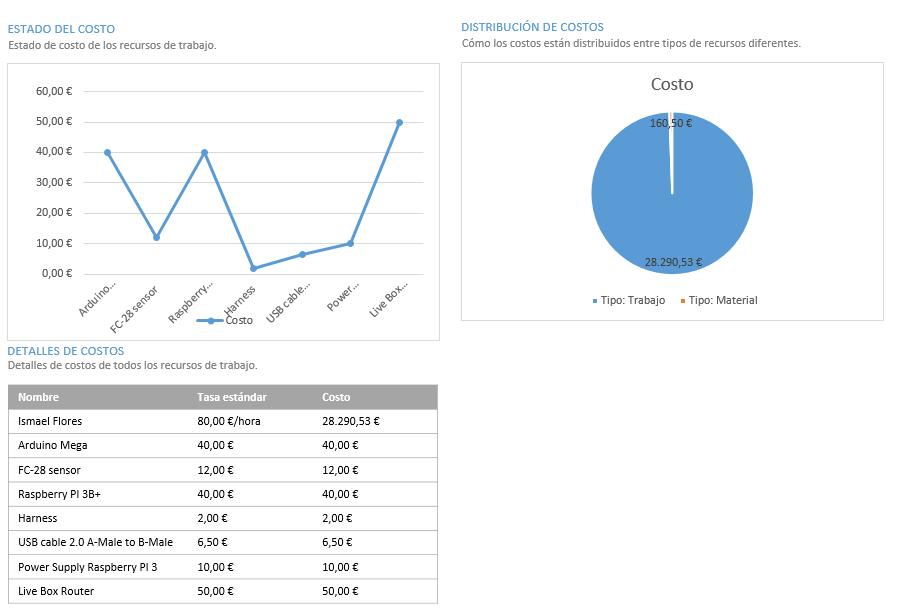
\includegraphics[scale=0.65]{IMGS/numbers_project.PNG}
\caption{Cost of the entire project \label{Cost of the entire project}}
\end{centering}
\end{figure}

\newpage

This picture displays the costs of components and workforce. The picture allows to know which resources are more expensive. The following points explain the disbursement of the resources:

\begin{itemize}

\item \textit{Workforce}. Represents the resource which has a higher disbursement, representing the \textit{99,44\%} of the budget of the project. The cost of this resource ascends to \textit{28.290,53\euro}.

\item \textit{Physical components}. Represents the resource with the lower disbursement, ascending to the \textit{0,56\%} of the budget of the project. The cost of the physical components of the project is \textit{160,50\euro}.

\end{itemize}

With the commented information, it is understood which resources required to invest a higher disbursement. The workforce represents the higher values of the cost of the project. The cost per hour of the employee ascends to \textit{80\euro per hour}, value which represents a standard value for a Computer Engineer in Germany. This information allows to understand where is important to invest when it is required to develop a customized solution for a client. Normally, the price of the projects are not bounded to the required hardware.\\

This information allows to understand where goes the budget in projects. In the following picture it is represented the cost of the different physical components of the project:

\begin{figure}[H]
\begin{centering}
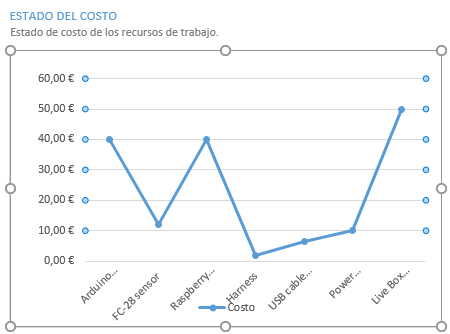
\includegraphics[scale=1]{IMGS/cost_materials.PNG}
\caption{Cost of the physical componets \label{Cost of the physical componets}}
\end{centering}
\end{figure}

This graph allows to have an overview about the cost of the physical components. The most expensive component is the product Live Box router reaching 50\euro. This price is nothing compared to the value of the workforce required to develop the system.

The workforce is the resource which has the highest value in projects.

\newpage
\newpage